\chapter{Desarrollo de la Aplicación}
\label{desarrollo-capitulo}

En el presente capítulo se presenta, de forma detallada, cómo fue el desarrollo del proyecto, los objetivos y actividades específicas de cada \textit{Sprint} y finaliza con una revisión de dificultades técnicas y los resultados del proyecto.

\section{Fase de Preparación}
    \subsection{Primer Sprint}
    
    En este \textit{sprint} se realizó las descargas de herramientas y la creación de los diagramas que serán la guía de desarrollo del sistema.
    
    \begin{enumerate}
        \item Objetivos
        \begin{enumerate}
            \item Levantar los requerimientos del producto.
            \item Documentación de la aplicación.
            \item Introducción al ambiente de trabajo.
        \end{enumerate}
        \item Actividades
        \begin{itemize}
            \item Creación del \textit{Product Backlog}
            \item Documentar la aplicación.
            \item Creación del diagrama ER-E para la base de datos de la aplicación.
            \item Creación de un modelo de casos de uso de la aplicación.
            \item Descarga de las herramientas ya mencionadas en el marco tecnológico.
        \end{itemize}
    \end{enumerate}
        
\section{Fase de Desarrollo}
    
    \subsection{Primer Sprint: Configuración de la aplicación}
    
    En este \textit{sprint} se configuraron Eclipse, Apache y MySQL para crear un ambiente de desarrollo adecuado para el sistema a desarrollar.
    
    \begin{enumerate}
        \item Objetivos
        \begin{enumerate}
            \item Crear y configurar el ambiente de desarrollo
            \item Descargar y configurar las herramientas necesarias para el desarrollo
            \item Descargar y configurar las herramientas necesarias para la gestión del proyecto         
        \end{enumerate}
        \item Actividades
        \begin{itemize}
            \item Creación de cuenta y tablas en Trello para la gestión del proyecto
            
            Las tablas de notas usadas fueron ``Pendiente", ``Impedido", ``En desarrollo" y ``Tarminado"; para referirse al estado actual de las tareas en cada una de las listas.
            
            \item Creación de repositorios
            
            Se crearon los repositorios Git tanto local como remoto, para el almacenamiento de la aplicación usando Git y Github como sitio de almacenamiento para los repositorios remotos. Los repositorios están bajo los nombres de ``ocupacional" y ``proyectoAngular" en el url: \textit{www.github.com/atarazona89}.
            
            \item Diseño de la Base de Datos
            
            Creación del diagrama ER-E y el glosario de términos de la aplicación. Ver apéndice \ref{ere}.
            
            \item Descarga del \textit{IDE} Eclipse
            
            Para el desarrollo se utilizo Eclipse Kepler, descargado de la página oficial de Eclipse\cite{ECLIPSE-eclipseorg}
            
           \item Descargar y configurar \textit{plugins} de Eclipse
           
           Se realizaron los cambios necesarios en la configuración del ``pom.xml" para así acceder a los repositorios de Maven que contienen las distintas librerías tanto de SPRING como de las distintas herramientas ya mencionadas. Se realizó la depuración de los archivos y la respectiva configuración adecuada al ambiente de trabajo. Esto se refiere a la configurar Eclipse para usar \textit{SPRING} como \textit{framework}, Hibernate y Liquibase como gestores de comunicación con la base de datos y configurar la base de datos con las credenciales de MySQL asignadas para el desarrollo del proyecto.
           
           \begin{table}[h!]
               
               \begin{center}
                   \begin{tabular}{|l|l|l|}\hline
                       Grupo & Artefacto & Versión \\\hline
                       org.springframework & spring-core & 4.1.2.RELEASE \\\hline
                       org.springframework & spring-orm & 4.1.2.RELEASE \\\hline
                       org.springframework & spring-webmvc & 4.1.2.RELEASE \\\hline
                       mysql & mysql-connector-java & 5.1.9 \\\hline
                       org.liquibase & liquibase-plugin & 1.6.1.0 \\\hline
                    \end{tabular}
                \end{center}
                
                \caption{Artefactos de Maven: Spring}
                \label{artefactos-spring}
           \end{table}
            
           Aunque, en lo referente a liquibase, se utilizó un plugin, no una librería. Ver cuadro \ref{artefactos-hibernate}.
           
           \item Configuración de las características de \textit{SPRING} para trabajar con anotaciones
           
           Se realizaron los cambios dentro del archivo ``occupational-servlet.xml" que permiten el uso de anotaciones para el direccio amiento interno de los procesos.
           
           
           \item Descargar y configurar la librería de JSON para la comunicación con el \textit{front-end}
           
           Usando los repositorios de Maven se descargaron las librerías necesarias de JSON para la comunicación. Las dependencias descargadas fueron, del grupo \textit{com.fasterxml.jackson.core}, las enumeradas en el cuadro \ref{artefactos-json}.
           
           \begin{table}[h!]
               
               \begin{center}
                    \begin{tabular}{|l|l|}\hline
                       Artefacto & Versión \\\hline
                       jackson-core & 2.2.2 \\\hline
                       jackson-annotations & 2.2.2 \\\hline
                       jackson-databind & 2.2.2 \\\hline                   
                    \end{tabular}
                \end{center}
                
                \caption{Artefactos de Maven: JSON}
                \label{artefactos-json}
            \end{table}
           
           \item Descargar y configurar las librerías de Hibernate para la comunicación con la base de datos
           
           Usando Maven fueron descargadas las librerías de Hibernate que usan JPA como API para comunicarse con la base de datos.
           
           \begin{table}[h!]
               
               \begin{center}
                   \begin{tabular}{|l|l|l|}\hline
                       Grupo & Artefacto & Versión \\\hline
                       org.hibernate.javax.persistence & hibernate-jpa-2.0-api & 1.0.1.Final \\\hline
                       org.hibernate.common & hibernate-commons-annotations & 4.0.4.Final \\\hline
                       javax.persistence & persistence-api & 1.0.2 \\\hline
                       org.hibernate & hibernate-entitymanager & 4.1.9.Final \\\hline
                       org.springframework.data & spring-data-jpa & 1.8.1.RELEASE \\\hline
                    \end{tabular}
                \end{center}
                
                \caption{Artefactos de Maven: Hibernate}
                \label{artefactos-hibernate}
            \end{table}
           
        \end{itemize}
    \end{enumerate}
        
        
    \subsection{Segundo Sprint: Configuración de la aplicación}
    
    En este \textit{sprint} se relizaron las configuraciones necesarias de las herramientas y la creación de funcionalidades básicas del lado del servidor para empezar el desarrollo del sistema.
    
    \begin{enumerate}
        \item Objetivos
        \begin{enumerate}
            \item Creación de clases, repositorios y servicios básicos.
            \item Creación de controladores básicos.
        \end{enumerate}
        \item Actividades
        \begin{itemize}
            \item Crear las siguientes clases para manejo de la información:
            \begin{itemize}
                \item Usuario
                \item Paciente
                \item Doctor
                \item Empresa
                \item Centro de Costos
                \item Sede
                \item Departamento
                \item Consulta
                \item Nota de revisión (\textit{SoapNote}, por \textit{Subjective, Objective, Assessment, Plan})
                \item Diagnóstico
                \item Examen
                \item Consulta
                \item Récipe
                \item Medicamento
                \item Laboratorio
            \end{itemize}
            
            \item Crear los repositorios
            
            En este entorno `repositorios' se refiere a las interfaces que usa \textit{Hibernate} para manejar los accesos y consultas con la base de datos. Estos repositorios vienen con métodos y procedimientos  implemantados por Hibernate y estipulados por JPA.
            
            Se creó un paquete de clases, llamado ``repositories", con un repositorio para cada una de las clases mencionadas anteriormente.
             
            \item Crear los servicios para las clases
            
            Los servicios están compuestos por una interfaz y su respectiva implementación por cada una de las clases mencionadas. Estos servicios se encargan de procesar la información haciendo uso de los repositorios, en caso de ser necesario, para brindar respuestas encapsuladas a los respectivos controladores.
            
            \item Crear los controladores de la aplicación
            
            En este \textit{Sprint} se crearon los controladores con operaciones básicas de gestión (crear, listar, consultar, modificar y eliminar) de cada una de las clases, dejando para futuros \textit{Sprint} la tarea de modificar los mismos las tareas específicas, en caso de ser necesario.
            
        \end{itemize}
    \end{enumerate}
        
        
    \subsection{Tercer Sprint: Autenticación y gestión de Usuarios}
    
    En este \textit{sprint} se implementó el módulo de autenticación y las funcionalidades básicas de gestión de usuarios, dejando para el siguiente \textit{sprint} la parte estética de dicha gestión.
    
    \begin{enumerate}
        \item Objetivos
        \begin{enumerate}
            \item Implementación de la autenticación basada en tokens.
            \item Creación, consulta, edición y eliminación de usuarios.
        \end{enumerate}
        \item Actividades
        \begin{itemize}
            \item Se implementó el módulo de autenticación siguiedo los parámetros de autenticación basada en \textit{tokens}
            La clave usada por el servidor fue una clave generada en tiempo de ejecución para que la misma fuera cambiante y mejorar la seguridad. Sin embargo, la clave, una vez generada se mantiene igual mientras el servidor esté en funcionamiento. Ver figura \ref{Autenticación}.
            
            \begin{figure}[htbp!]
                \begin{center}
                    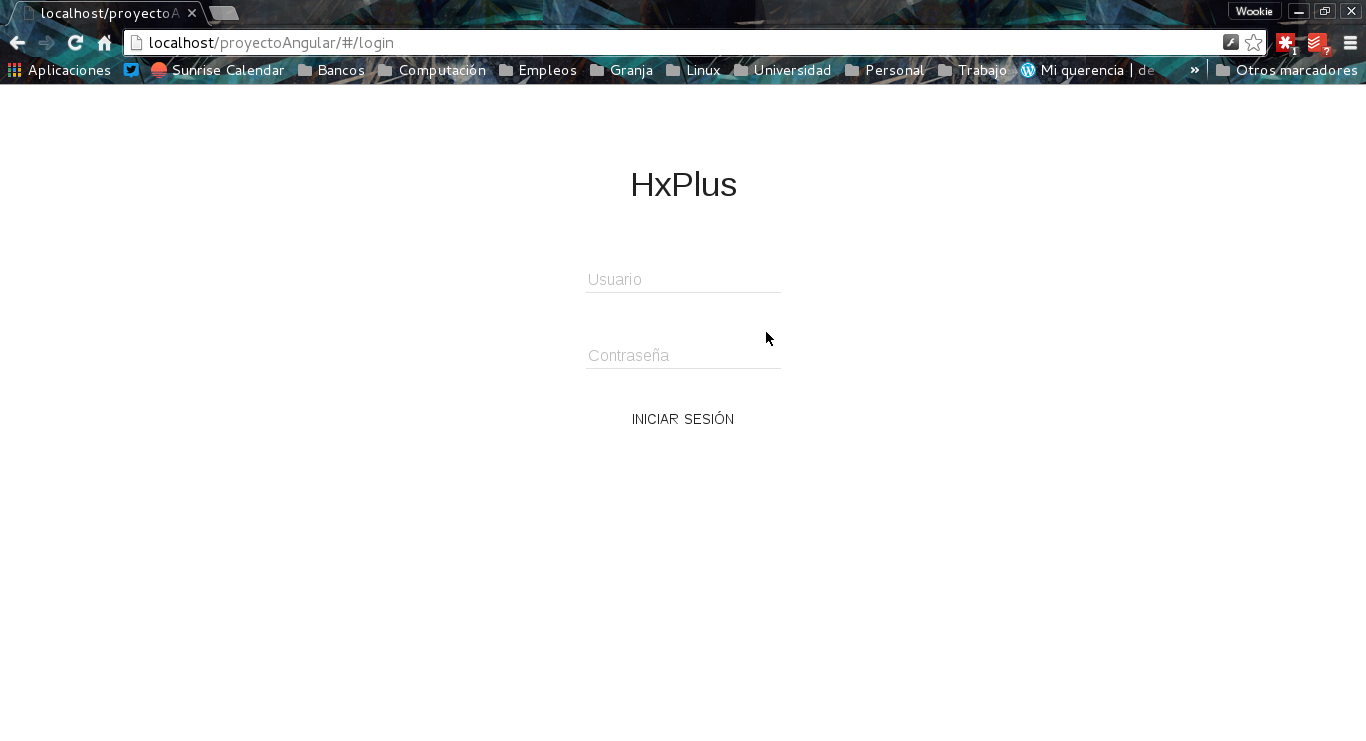
\includegraphics[width=.8\textwidth]{figures/p1}
                \end{center}
                \caption{Pantalla de Autenticación de usuarios}
                \label{Autenticación}
            \end{figure}
            
            Para ello se agregó al ``pom.xml" las dependencias requeridas para la autenticación. Ver cuadro \ref{artefactos-tba}
            
            \begin{table}[h!]
                
                \begin{center}
                    \begin{tabular}{|l|l|l|}\hline
                        Grupo & Artefacto & Versión \\\hline
                        io.jsonwebtoken & jjwt & 0.5.1 \\\hline
                    \end{tabular}
                \end{center}
                
                \caption{Artefactos de Maven: Autenticación}
                \label{artefactos-tba}
            \end{table}
            
            \item Se implementó el módulo de gestión de usuarios, en el mismo, un usuario, con las credenciales adecuadas, puede crear, usuarios nuevos y se despliega una lista de los usuarios en la  cual se puede elegir uno para luego poder editarlo o eliminarlo definitivamente de la base de datos. Esta última acción no es reversible por lo cual queda a consideración del \textit{Product Owner} si quedará finalmente la funcionalidad al alcance de los usuarios. Ver figuras \ref{Revisión} y \ref{Edición}.
            
            \begin{figure}[htbp!]
                \begin{center}
                    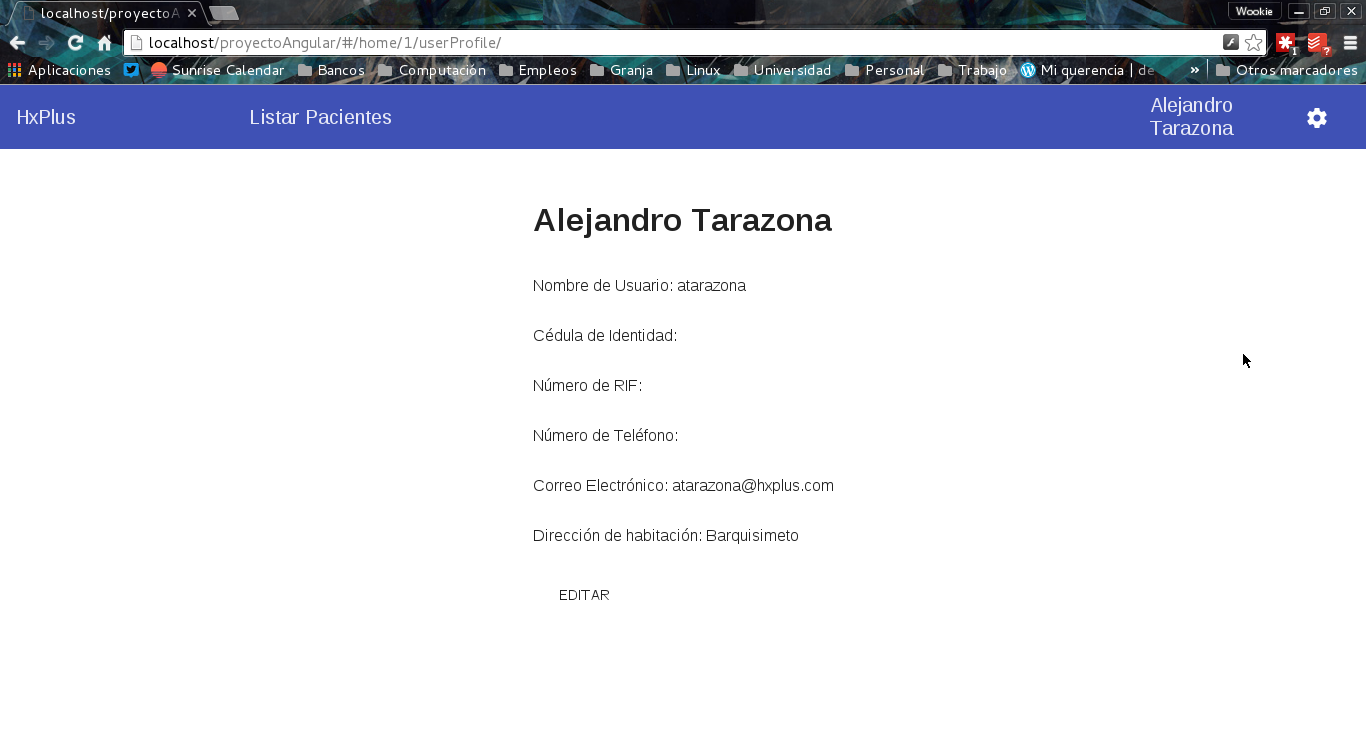
\includegraphics[width=.8\textwidth]{figures/p3}
                \end{center}
                \caption{Pantalla de Revisión de Usuario.}
                \label{Revisión}
            \end{figure}
            
            \begin{figure}[htbp!]
                \begin{center}
                    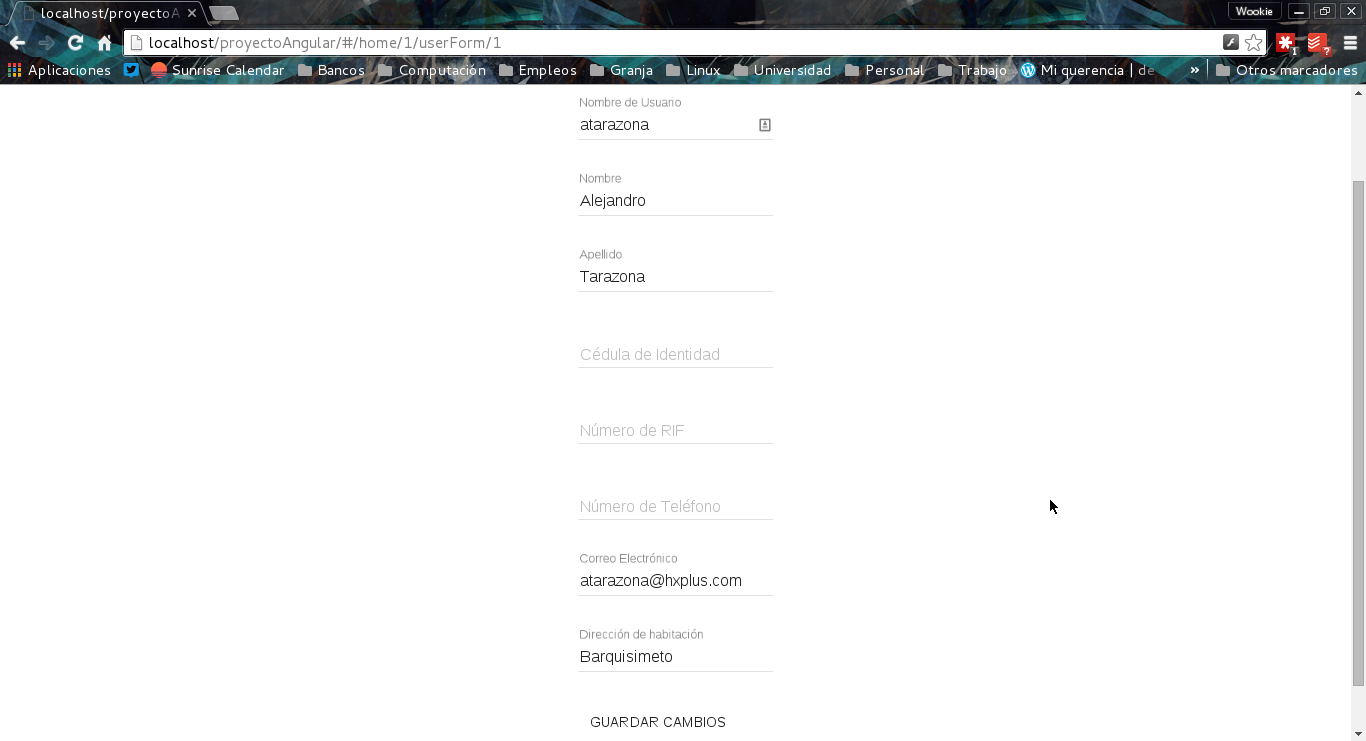
\includegraphics[width=.8\textwidth]{figures/p5}
                \end{center}
                \caption{Pantalla de Edición de Usuario.}
                \label{Edición}
            \end{figure}
            
        \end{itemize}
         

         
            
    \end{enumerate}
             
        
    \subsection{Cuarto Sprint: Consultas de Usuarios y Vista del doctor}
    
    En este \textit{sprint} se mejoró la estética de la lista de usuarios y se implementó la visualización de parte de los doctores.
    
    \begin{enumerate}
        \item Objetivos
        \begin{itemize}
            \item Consultas del módulo de usuarios.
            \item Desarrollo de la vista del doctor.
        \end{itemize}
        \item Actividades
        \begin{itemize}
            \item Ordenamiento de las listas de usuarios
            
            La lista de usuarios implementada en el \textit{sprint} anterior fue reordenada para aparecer alfabéticamente en pantalla. Las funcionalidades previas no fueron modificadas.
            
            \item Visualización de usuarios
            
            La lista también fue modificada para que fuese visualizada con apariencia de lista de usuarios siguiendo los lineamientos de Material Design. Ver figura \ref{Pacientes}.
            
            \begin{figure}[htbp!]
                \begin{center}
                    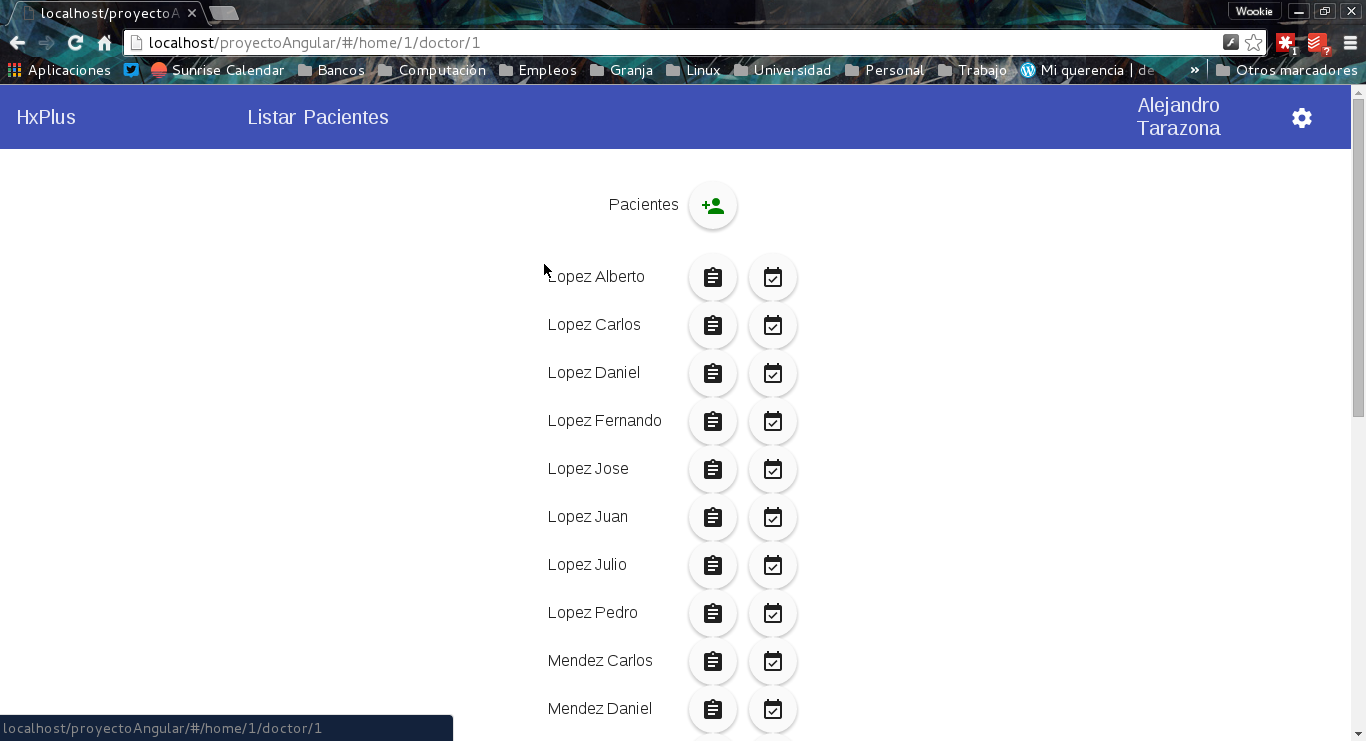
\includegraphics[width=.8\textwidth]{figures/p6}
                \end{center}
                \caption{\label{Pacientes}Lista de Pacientes del Médico}
            \end{figure}
            
            \item Creación de la vista del doctor
            
            Esta incluye la lista de pacientes a atender en el día actual y la lista de pacientes que ha atendido el doctor. Junto con las funcionalidades de:
            
            \begin{itemize}
                \item Agregar Paciente: Agrega un paciente nuevo a la lista de doctor, ya sea tomado de la lista de pacientes (Tal como se muestra en la figura \ref{Agregar}) o creando un nuevo historial y agregándolo inmediatamente a la lista de pacientes del doctor (Figura \ref{creación}).
                
                \begin{figure}[htbp!]
                    \begin{center}
                        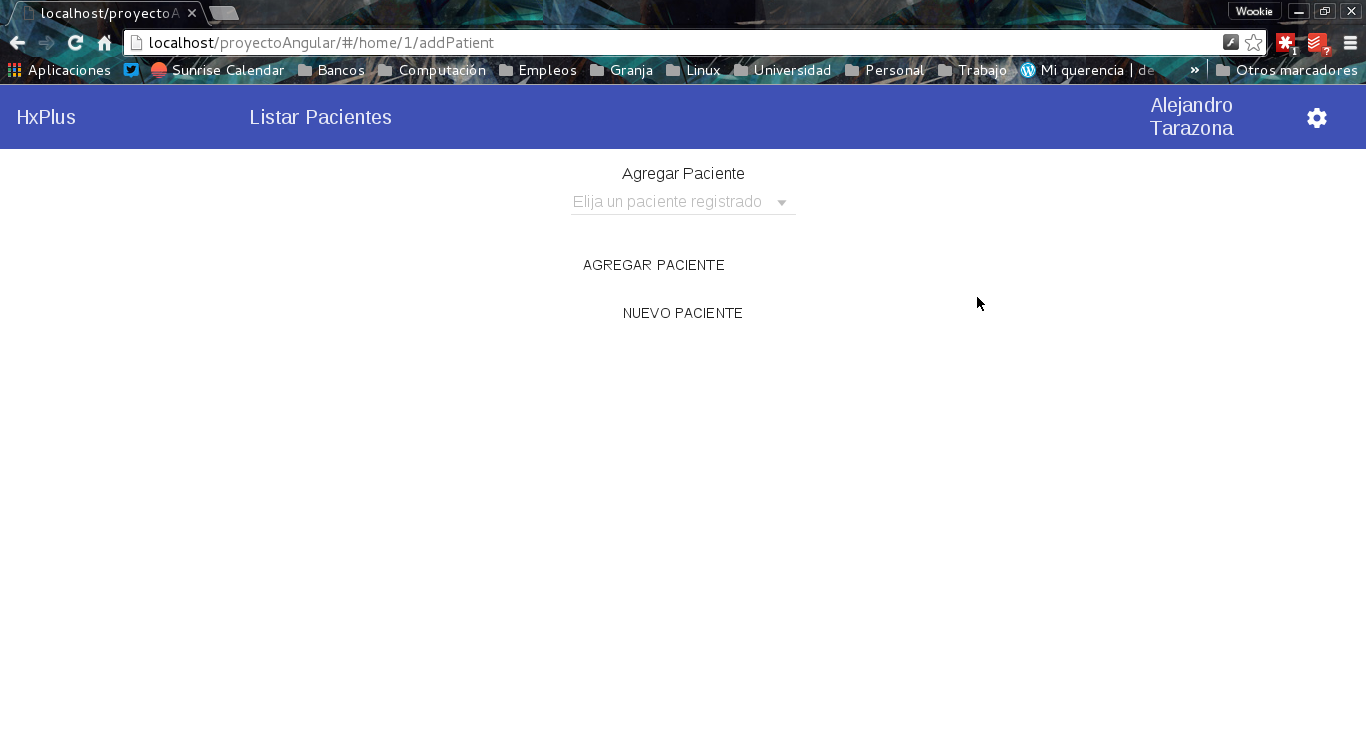
\includegraphics[width=.8\textwidth]{figures/p8}
                    \end{center}
                    \caption{Vista de Agregar pacientes que ya han sido atendidos por algún médico.}
                    \label{Agregar}
                \end{figure}
                
                \begin{figure}[htbp!]
                    \begin{center}
                        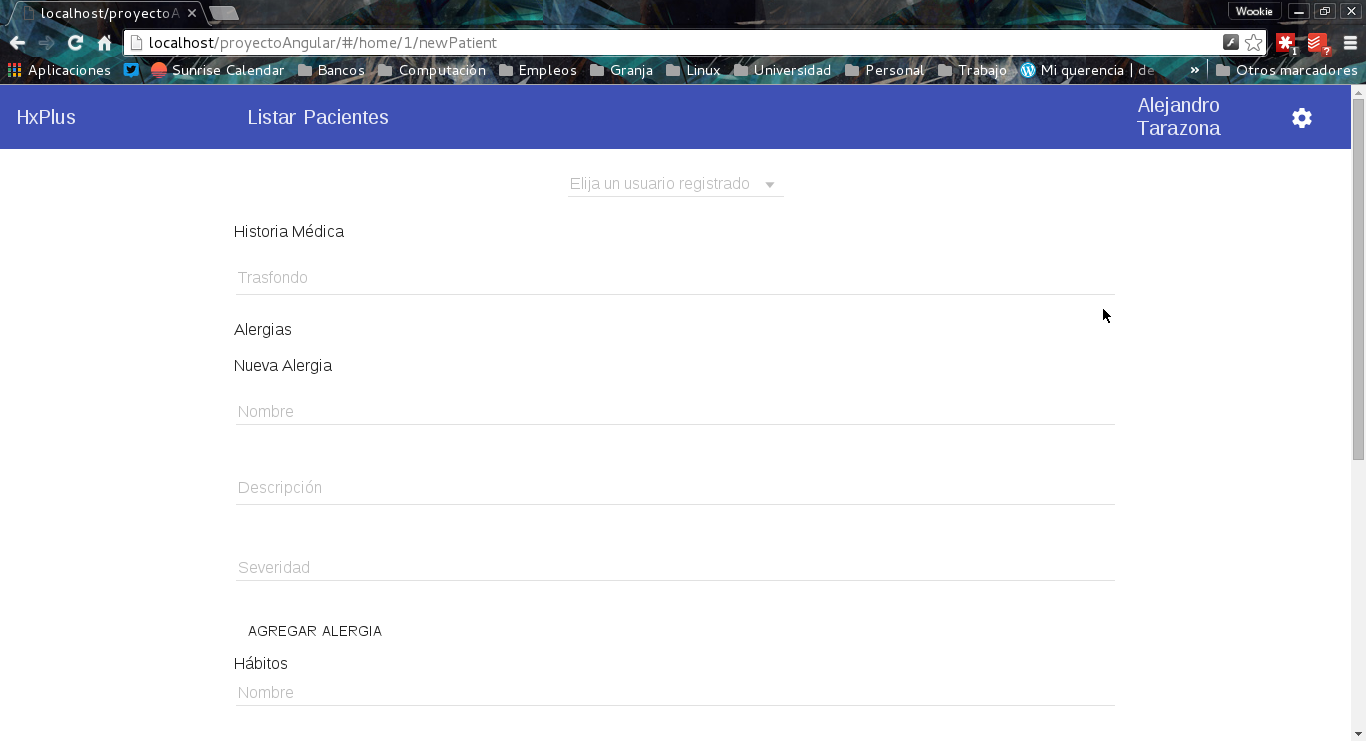
\includegraphics[width=.8\textwidth]{figures/p10}
                    \end{center}
                    \caption{Vista de creación de nueva historia médica para un paciente nuevo.}
                    \label{creación}
                \end{figure}
                
                \item Crear Consulta: Crea una nueva consulta al historial de paciente. En este \textit{sprint} se realizó la funcionalidad de ``programar" una confulta futura, que permitirá la planificación de consultas. Se dejó para un futuro \textit{sprint} la ceración de la consulta en sí misma ya que amerita el manejo de otros tipos de datos adicionales.
            \end{itemize}           
            
            No se implementó la funcionalidad de ``Eliminar Paciente" ni la de ``Modificar Paciente" dado que el sistema busca mantener un registro histórico de las consultas y un médico no debería poder modificar ni eliminar dicho registro, sólo agregar nueva información al mismo.
            
        \end{itemize}

    \end{enumerate}
        
        
    \subsection{Quinto Sprint: Consulta del Paciente}
    
    En este \textit{sprint} se implementó el módulo de consultas del paciente, en este módulo el doctor puede crear y almacenar los datos pertinentes a una consulta dada y los mismos serán agregados al historial médico del paciente.
    
    \begin{enumerate}
        \item Objetivos
        \begin{itemize}
            \item Generación de consultas.
            \item Gestión de la linea de tiempo de la consulta del paciente.
        \end{itemize}
        \item Actividades
        \begin{itemize}
            \item Crear consulta nueva
            
            Se crea la nueva consulta, permitiendo a médico almacenar los datos pertinentes. La consulta creada se agrega inmediatamente al historial del paciente, anexando los diagnósticos, en caso de haberlos, a su apartado exclusivo dentro del historial.
            
            Se almacenan los signos vitales o parámetros fisiológicos pertinentes, peso, estatura, tensión arterial entre otros. Se deja libertad al médico para añadir nuevos parámetros a los que ya estén almacenados en la base de datos (Figura \ref{parametros}).
            
            \begin{figure}[htbp!]
                \begin{center}
                    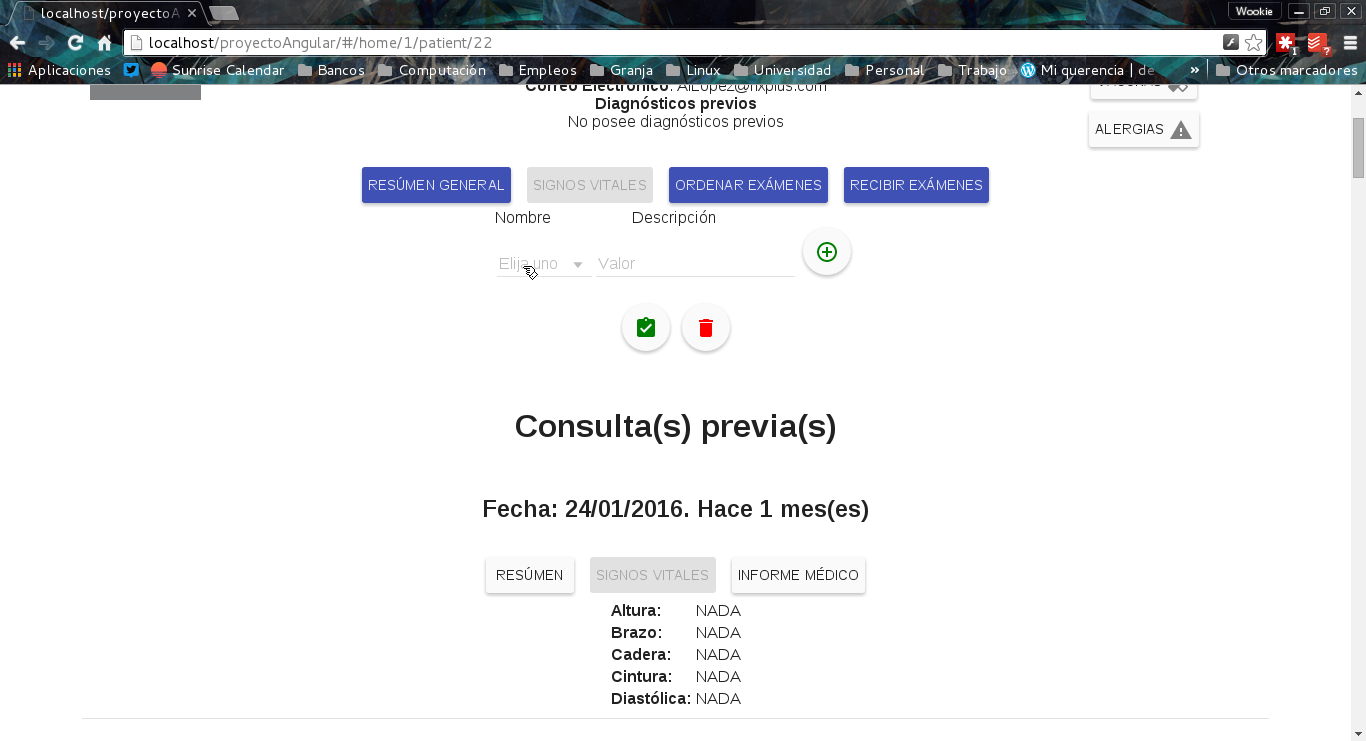
\includegraphics[width=.8\textwidth]{figures/p13}
                \end{center}
                \caption{\textit{Paarámetros Fisiológicos}}
                \label{parametros}
            \end{figure}
            
            \item Creación de \textit{Soap Note}
            
            Se crea y almacena, para cada consulta, los datos recogidos en la consulta (Figura \ref{soapnote}). Tales son:
            
            \begin{itemize}
                \item \underline{Subjetivos (\textit{Sbjective}):} Lo que el paciente atestigua, sintomas y comentarios hechos por el paciente en el lenguaje que el mismo paciente los exprese para así mantener la información sin cambios en caso de que sea necesario revisarlos.
                \item \underline{Objetivos (\textit{Objective}):} Lo que el médico puede observar en la consulta. Se usa en esta sección el lenguaje técnico propio de la medicina.
                \item \underline{Comentarios (\textit{Assessment})}: Algún comentario u obsevación adicional que pueda hacer el doctor.
                \item \underline{Plan:} Se acordó que el \textit{Plan} estaría en un apartado especial por cuestiones de simplicidad y acceso a los datos.
            \end{itemize}
            
            \begin{figure}[htbp!]
                \begin{center}
                    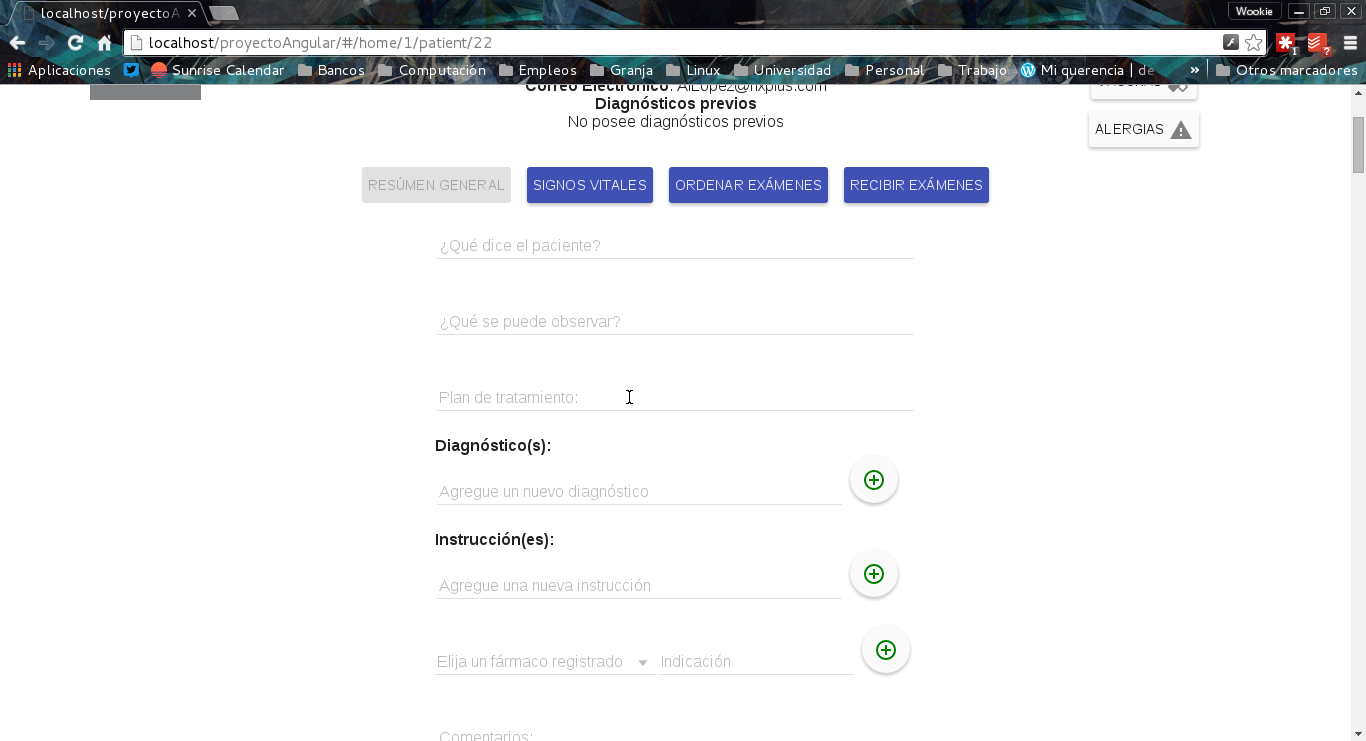
\includegraphics[width=.8\textwidth]{figures/p12}
                \end{center}
                \caption{\textit{Soap Note}}
                \label{soapnote}
            \end{figure}
            
            \item Solicitud y recepción de exámenes médicos
            
            El médico  tratante tiene uns sección de solicitud de exámenes médicos. En ella indica el nombre del exámen a solicitarle al paciente (Figura \ref{solicitudExamen}) Estas solicitudes quedan almacenadas y en futuras consultas, el médico tiene la opción de indicar la recepción de algún exámen previamente solicitado, ya sea uno o varios de ellos (Figura \ref{recepcionExamen}).
            
            \begin{figure}[htbp!]
                \begin{center}
                    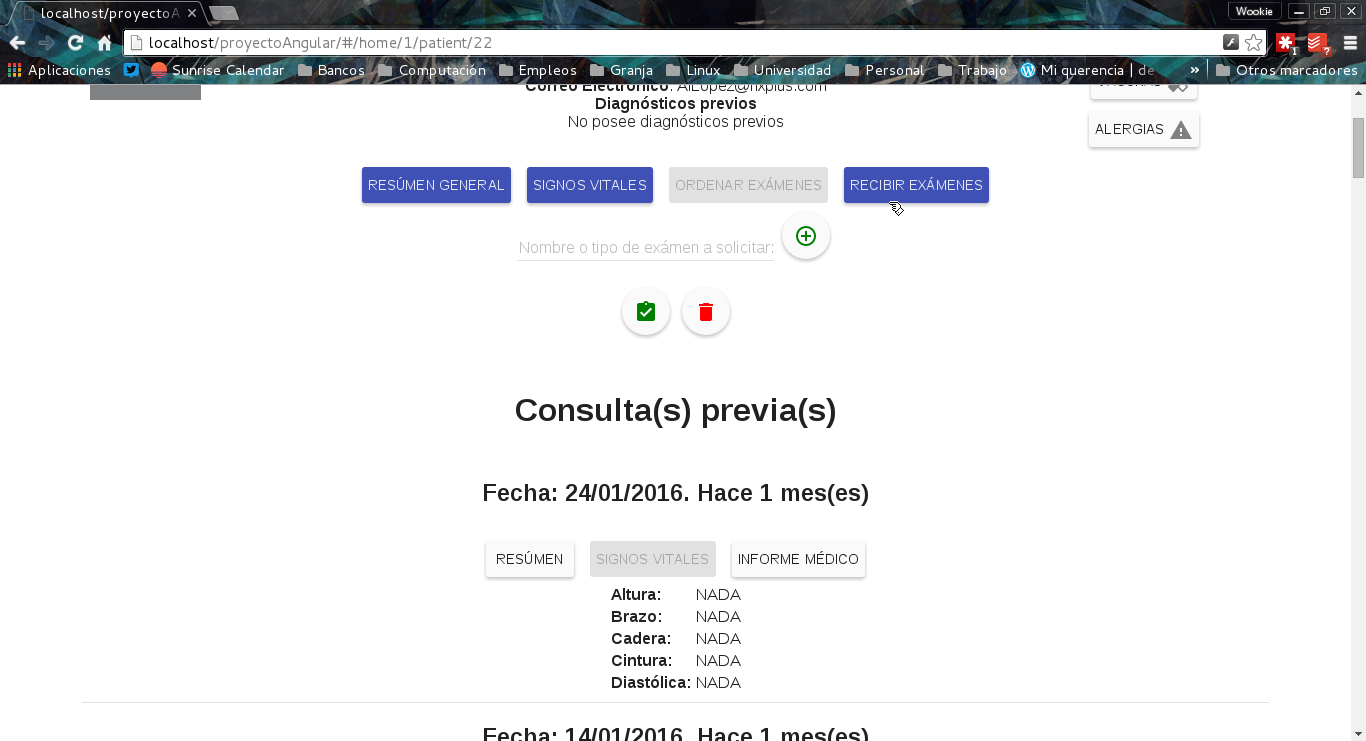
\includegraphics[width=.8\textwidth]{figures/p16}
                \end{center}
                \caption{\textit{Solicitud de Exámenes}}
                \label{solicitudExamen}
            \end{figure}
            
            \begin{figure}[htbp!]
                \begin{center}
                    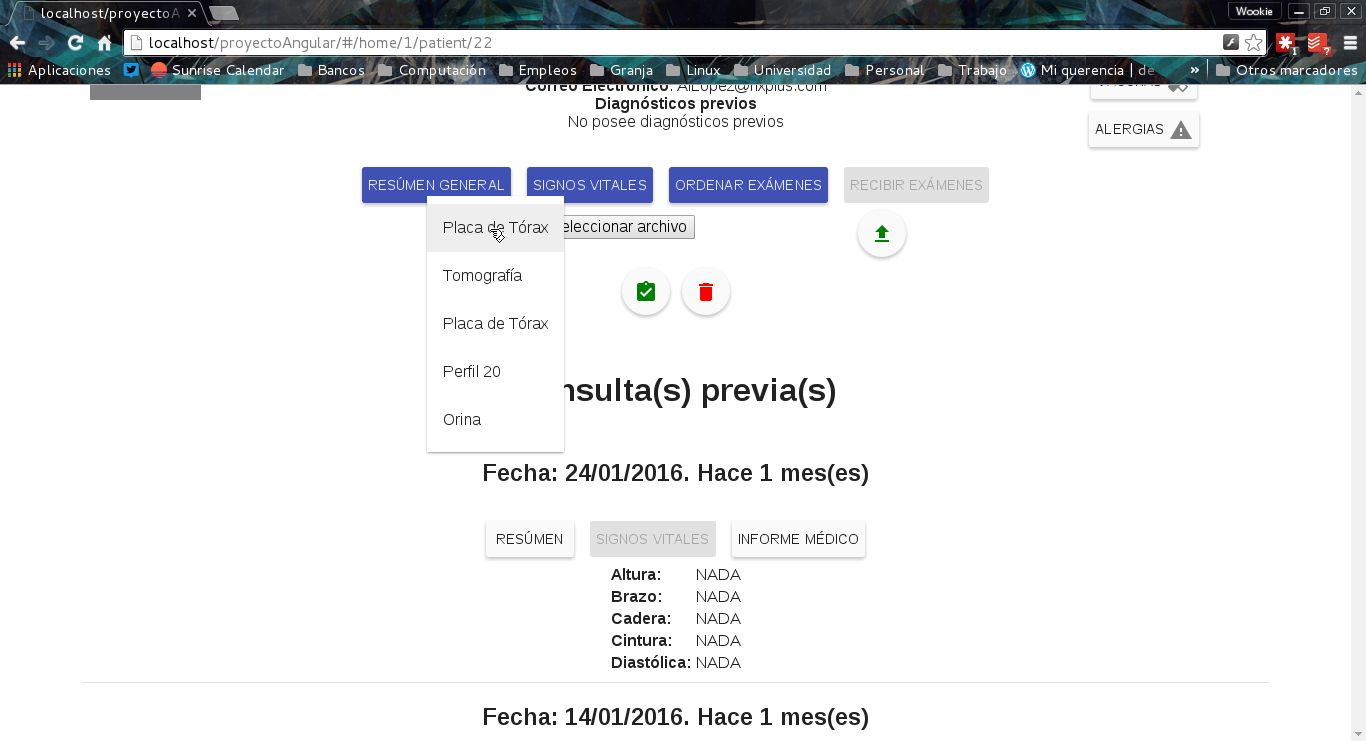
\includegraphics[width=.8\textwidth]{figures/p17}
                \end{center}
                \caption{\textit{Recepción de Exámenes}}
                \label{recepcionExamen}
            \end{figure}
            
            En la sección de recepción de exámenes, el médico también tiene la opción de adjuntar algún archivo, ya sea resultados (en el caso de exámens sanguíneos) o imágenes (ecografías, rayos X, etc) los cuales serán anexados a la respectiva consulta y con ella al historial del paciente.
            
            \item Creación de diagnósticos
            
            El médico también puede almacenar uno o varios diagnósticos por consulta, estos constan de un nombre de enfermedad o dolencia y una gravedad. Ello lo elige de listas desplegables que estarán a su disposición tomando la base de datos del sistema. También se le permite agregar un nuevo diagnóstico en caso de carecer de ello el sistema, y el mismo será almacenado con posibilidad de reutilización (sólo del nombre) en futuras consultas.
            
            \item Creación del plan de tratamiento
            
            El médico puede crear un plan de tratamiento, el cual consiste en:
            \begin{itemize}
                \item Recomendaciones: Cambios o hábitos de los que el paciente deba cuidarse, así como recomendaciones alimenticias y reposos. Es una sección informal.
                \item Comentarios: Algun comentario extra, preguntas o anotaciones que el médico quiera hacer del conocimiento del paciente.
                \item Tratamiento: Este incluye al menos un medicamento y la posología elegida para cada uno de los medicamentoa añadidos. Los medicamentos son elegidos de la base de datos del sistema. El administrador del sistema se encararía de añadir o eliminar medicamentos a la base de datos por ahora.
                \item Récipe Médico: En este se indica un medicamento y su respectiva dosis para permitir al paciente su compra en la farmacia de su preferencia.
            \end{itemize}
            
            Esta información estará disponible, en un futuro \textit{Sprint} para ser impresa en hojas, según el formato lo establezca, y ser entregada al paciente.
            
        \end{itemize}
    \end{enumerate}
        
        
    \subsection{Sexto Sprint: Generar informes}
    \begin{enumerate}
        \item Objetivos
        \begin{itemize}
            \item Generación de informes médicos y reposos.
        \end{itemize}
        \item Actividades
        \begin{itemize}
            \item Investigar las herramientas disponibles para generar archivos PDF.
            \item Evaluar la compatibilidad con las herramientas y el \textit{framework} que se está usando en el dessarrollo de \textit{HxPlus Ocupacional}.
            \item Elegir una de las herramientas y realizar los cambios adecuados para su uso en el sistema. Para \textit{HxPlus Ocupacional} se eligión iText por las razones mencionadas anteriormente.
        \end{itemize}
    \end{enumerate}
        
    \subsection{Septimo Sprint: Generar informes}
    \begin{enumerate}
        \item Objetivos
        \begin{itemize}
            \item Vista de Solicitud de informes.
        \end{itemize}
        \item Actividades
        \begin{itemize}
            \item Se implantó la vista de solicitud de informes médicos con posibilidad de selección múltiple. Los parámetros son:
            \begin{itemize}
                \item Examen físico
                \item Diagnóstico(s)
                \item Tratamiento
                \item Comentario(s)
            \end{itemize}
            
            Tal como se muestra en la figura \ref{solicitudInforme}. Esto permite que en un solo formulario, el médico tiene la posibilidad de generar tanto informes como reposos médicos.
            
            \begin{figure}[htbp!]
                \begin{center}
                    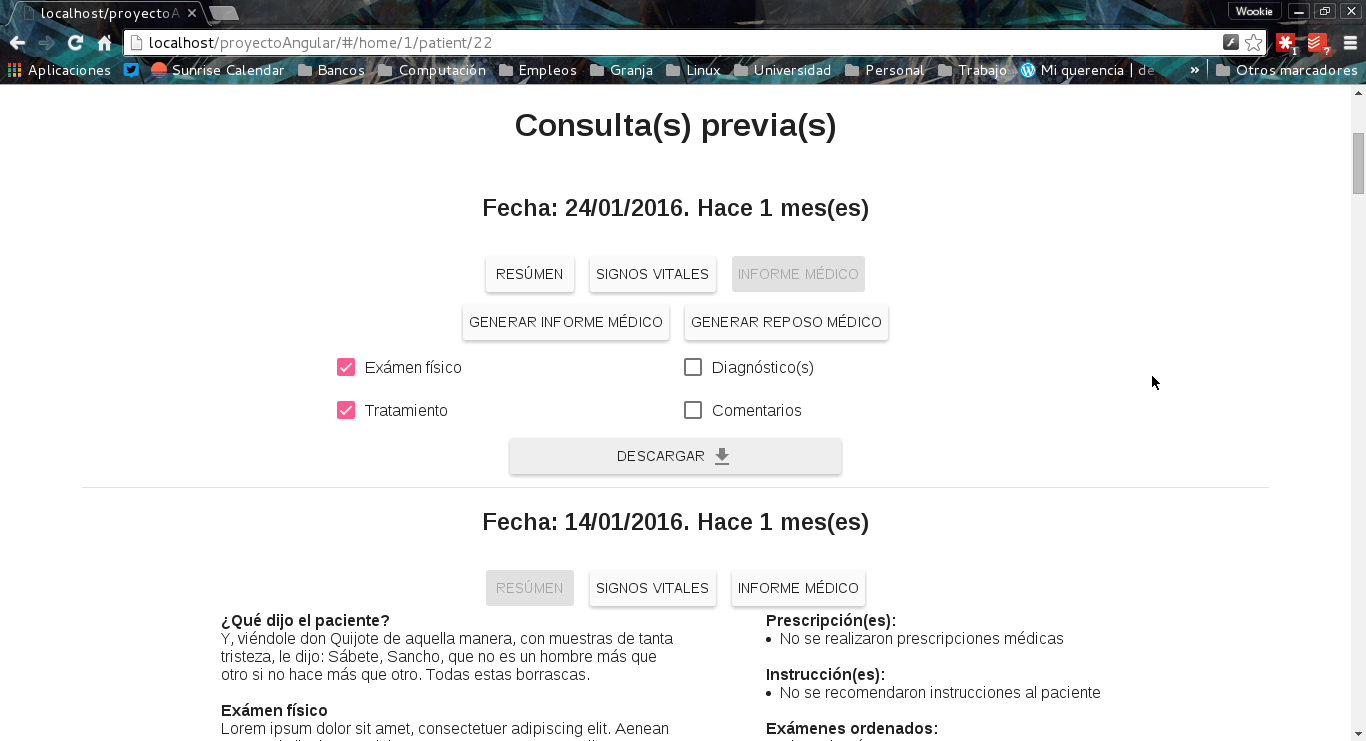
\includegraphics[width=.8\textwidth]{figures/p23}
                \end{center}
                \caption{Sección de solicitud de informes médicos.}
                \label{solicitudInforme}
            \end{figure}
        \end{itemize}
    \end{enumerate}
        
        
    \subsection{Octavo Sprint: Generar informes}
    \begin{enumerate}
        \item Objetivos
        \begin{itemize}
            \item Generacion de informes.
        \end{itemize}
        \item Actividades
        \begin{itemize}
            \item Se implantó el módulo de generación de informes médicos, tal y como fue descrito anteriormente, usando los parámetros selecciónados se generó el informe respectivo usando el formato indicado. Ver figura \ref{informeModelo}.
        \end{itemize}
        
        \begin{figure}[htbp!]
            \begin{center}
                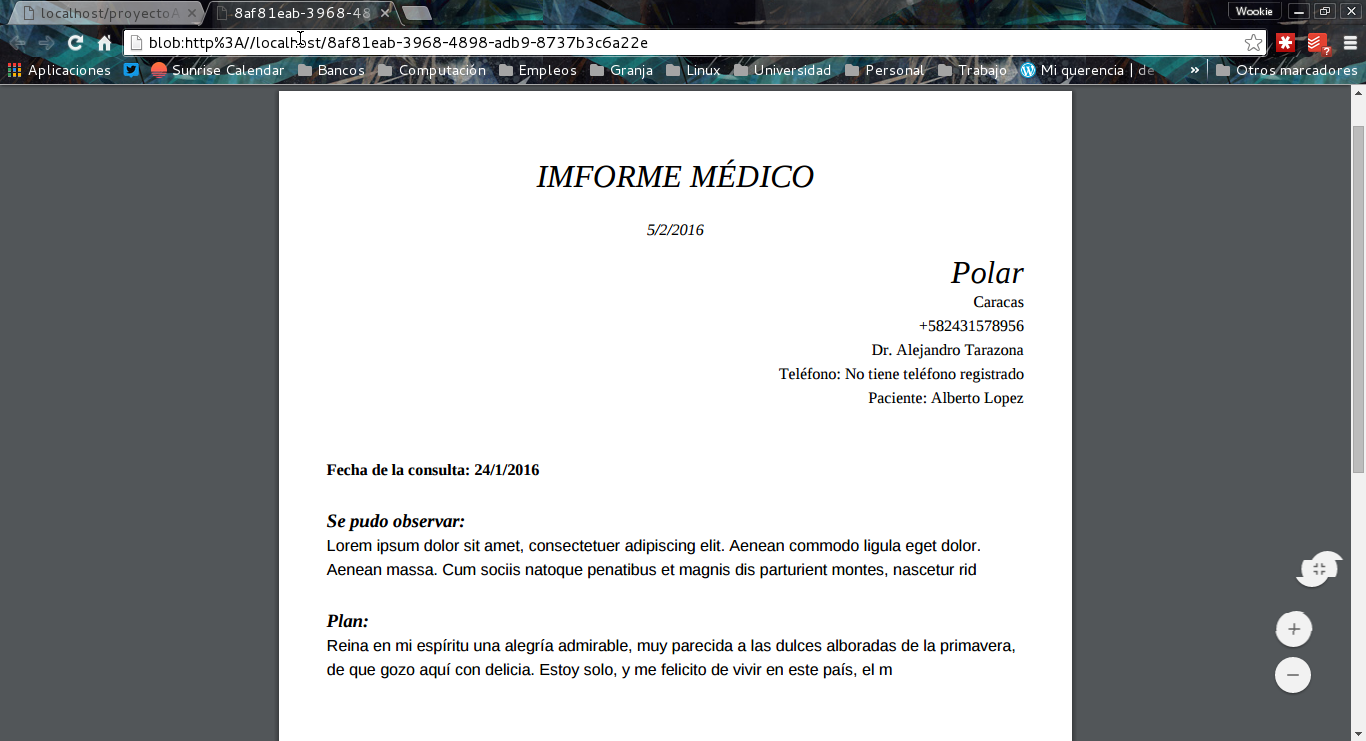
\includegraphics[width=.8\textwidth]{figures/p22}
            \end{center}
            \caption{Informe modelo}
            \label{informeModelo}
        \end{figure}
    \end{enumerate}
        
    
\section{Fase de Cierre}
    \subsection{Primer Sprint: Pruebas finales y puesta en producción}
    \begin{enumerate}
        \item Objetivos
        \begin{itemize}
            \item Resolución de incidencias.
            \item Diseño y ejecución de pruebas.
            \item Puesta en producción.
        \end{itemize}
        \item Actividades
        \begin{itemize}
            \item Se revisaron las incidencias y posibles errores de consistencia de la información y su acceso en el sistema.
            \item Se realizaron pruebas de aceptación de parte del \textit{Scrum Master} en el uso del sistema.
        \end{itemize}
    \end{enumerate}
        
    \subsection{Segundo Sprint: Redacción del libro de pasantías}
    \begin{enumerate}
        \item Objetivos
        \begin{itemize}
            \item Redacción del libro de pasantías.
            \item Revisión y culminación del libro de pasantías.
        \end{itemize}
        \item Actividades
        \begin{itemize}
            \item Se recopiló la información del proyecto
            \item Se realizó el filtrado de dicha información y se llevó al presente trabajo en limpio para su presentación.
        \end{itemize}
    \end{enumerate}
        
        
    \subsection{Dificultades generales encontradas}
    
    Las dificultades encontradas durante el desarrollo del proyecto fueron:
    
    \begin{itemize}
        \item \textbf{Restricción en el uso de herramientas:} el \textit{Product Owner} solicitó explícitamente el uso de Java, SPRING, Hbernate, JavaScript, MySQL, AngularJS y JSON, tal y como fue descrito, para el desarrollo. Lo cual, si bien facilitó la creación y desarrollo del proyecto, dejó imposibilitada la posibilidad de, con tecnologías actuales, dar soporte a una base de datos orientada a eventos, tal como se pretendía hacer en el principio, y no se logró este enfoque.
        
        \item \textbf{Falta de informción de parte de Inpsasel:} originalmente se buscaba generar informes médicos especializados para el reporte de enfermedades ocupacionales al Inpsasel, órgano encargado de la gestión de enfermedades ocupacionales en el émbito nacional. Sin embargo, la falta de información, formatos y, más adelante, el lanzamiento de su portal (de Inpsasel) con automatización de dicha gestión, dejó a HxPlus Ocupacional sin la necesidad de realizar dichos informes.
    \end{itemize}
    
    \subsection{Resultados Generales}
    
    El proyecto de pasantía se completó satisfactoriamente. A pesar de no poseer la funcioncionalidad de generación de informes de Inpsasel, la empresa de consideró satisfecha con los módulos implementados. La línea de tiempo de consultas se muestra adecuadamente y en orden cronológico, los diagnósticos y planes son almacenados y mostrados a gusto de la empresa y de conformidad con los lineamientos.
    
    Queda de parte de la empresa gestionar el desarrollo de futuros módulos o funcionalidades para la aplicación.
    
    
    
\pagebreak